\documentclass[12pt,a4paper,twocolumn]{article}
\usepackage{cite}
\usepackage{graphicx}
\usepackage{float}
\usepackage{subfig}
\begin{document}
\hyphenpenalty=10000
\tolerance=1000

\setlength{\parindent}{0mm}
\setlength{\parskip}{0.5 cm} 

\begin{titlepage}
\Large
{\center \bf BrikWorld}

\normalfont
\begin{flushright}
  {\em A Rollplaying Game}
\end{flushright}
\vspace{1cm}
\end{titlepage}

\normalsize
\section{Introduction}
Imagine a fantasy RPG with its eyes open.  A world whose narrative tropes not only exist independent of the actors that embody them, but are a well-documented and relied-upon force in their own right.  A world locked in war over the right to exploit natural resources, often against the wishes and over the dead bodies of those resources.  A world made almost entirely from interchangable plastic blocks.  This world is BrikWorld. 
\subsection{BrikWorld from a Distance}
Until a little more than six hundred years ago, BrikWorld was much like any other fantasy universe.  Heroes and Magic and Dungeons and Dragons fought continually over control of the land, to the land's great detriment.  Constant crisis ravaged the countryside and slaughtered the population, stopped only by the occasional band of stalwart adventurers.  The world teetered on the brink of extinction, kept from total darkness by tiny points of light.  This was the age of the Wild.

Funnily enough, in the end all it took to spark a sea change was a casual observation by a young mage named Arnold Heisenbrik.  In his words:
\begin{quote}
We are unable to determine at this time where the death beetle infestation came from.  There are no other entrances to the dungeon through which they may have come, no queen to lay eggs, and nothing to eat in there - until we excavated the single entrance.  The only explanation that admits itself is that the death beetles must have come from {\em nowhere} and eaten {\em nothing} until our party offered itself to be feasted upon, an idea so ridiculous I am uncertain whether to even mention it.
\end{quote}
Though Heisenbrik's Uncertain Principle was stated without the force of conjecture common to the time, it troubled other mages enough for them to verify it.  What Heisenbrik had unwittingly uncovered was an elemental force of Life, long thought to be a path for magic to flow along but now known to underpin nearly every part of the BrikWorld.

Within ten years, every major government was aware of the finding's implications - mages aren't any worse gossips than people generally are, but most are telepathic so news travels very fast.  Fifty years after that, it was common knowledge in any nation worth writing fluff for.

The world is still reeling.
\subsection{What to Expect from BrikWorld}
BrikWorld is a hybrid of roleplaying games with miniature wargames, cherrypicking the best of both worlds to make a unified experience.  As such, players from both genres are likely to encounter some new, unfamiliar, or at least really strange-sounding ideas.

\subsubsection{For Roleplayers}
The first and most obvious difference you'll notice is squad-level control.  Rather than pretending to be a single PC you'll be controlling groups of them, ranging in size from a handful of units to entire armies.  While you are welcome to name and ascribe unique personalities and desires to each of them if you'd like, and doing so usually turns out pretty cool, it is certainly not necessary and absolutely not required.  Naming your force as a whole and developing it along thematic lines are always good ideas though, so long as the name/theme isn't retarded.

As a player, you should never be required to roleplay in character.  You are not your units, but the mystical, invisible being watching over them and guiding their actions in a manner which they would approve of.  The decisions you make outside of combat reflect the combined will of your entire force, not the voices of only one or two.  Their tiny lives are in your incorporeal hands.  That said, a player might want to appoint one of her units as a "face," used principally for interaction with other groups, and speak mostly in character when strategizing.  That's fine too.  Just don't proposition other people's units.  That could get a little weird.

Finally, don't get too attached to your units.  BrikWars is a dangerous combat system where every hit is the equivalent of a save or die spell.  Although the chances of a TPK are low, any fight that's large enough to bother with will have at least a few casualties before it's won.  If you're the kind of person who can't stand seeing a beloved character pass on, you may want to start stocking up on healing potions now.  And try not to let other people know which mini is your favorite, just in case.

\subsubsection{For Wargamers}
Think of BrikWorld as a long campaign of small, easy battles, during which your force expands to meet a growing challenge. Completely losing a match is very unlikely, but it's easy to lose more units than the mission reward can replace.  Over time sub-par performance can make battles more difficult, and therefore more costly.  On the other hand, since the GM can and should somewhat tailor the enemy to your capabilities, army composition becomes less about optimum effectiveness and more about personal style. 

As you play, you'll be expected to think with the mindset of your army.  You don't have to pretend to be that army like it's some kind of improv theater, but try to make your decisions from their perspective.  Pretend they're real people.  Their loyalties are your loyalties.  Are they grizzled veterans, too combat-weary to care about anything but their survival?   Are they bright-eyed idealists ready to die for their town or nation?  Are they raw recruits, scared too shitless to do anything but catch bullets?  They're your boys, so it's your choice.

Most battles will be fought against a GM, who is also the person who sets the reward for the current mission's performance and decides which later missions your force has access to.  It may occur to you to wonder if there is a conflict of interest there.  The answer is "yes, yes there is."  The usual method for resolving GM disputes is to buy him pizza to make him fat and content and pray the issue never comes up to begin with.

Finally, although the GM might pit the players against each other if you make him angry enough, BrikWorld is largely a cooperative endeavor.  You're expected to work {\em with} your fellow players to achieve goals for a common benefit, even if they're too dumb to deserve it.  Especially if they're too dumb to deserve it, in fact, because standing back and letting them die will only make the next battle that much harder.

\subsection{Why BrikWars?}

Although any number of different wargaming mechanics might have been used to underpin our enterprise, we chose that of BrikWars for several of its more unique features:
\begin {itemize}
	\item Affordable.  Although the Lego miniatures that BrikWars was built to fight with are somewhat expensive, BrikWars itself is free, available at http://www.BrikWars.com, and does not depend on specific miniatures of any brand at all.
    \item Extensible.  BrikWars itself comes with its own advanced and self-contradictory set of rules, the 2001 rules, which are the product of half a decade of arguments, houserules and outright fistfights.  It's generally accepted that you can pick and choose which rules you like the most - virtually no one uses the default rules without alteration.  We'll suggest a small number of additional rules, but you're under no pressure to abide by them.  Use house rules, or someone else's house rules, or Cider House rules, or O'Doyle Rules.  Whatever floats your group's boat.
    \item Flexible.  In the default 2005 rules everything is the product of a smallish number of generic creation guidelines, balanced around miniature size and a point buy (CP) system.  If you get tired of minifig combat, play dragons vs. ogres, or use miniatures from another system - BrikWorld vs the Imperium of Man would make a damn fine campaign that practically writes itself.
	\item Casual.  BrikWars is above all a relaxed gameplay experience.  The only way to really play it wrong is to get upset at how the other people are playing.  Unless they're cheating or something, in which case don't give them any more beer until they stop.  That's another thing.  You must have beer.  Doing it sober is doing it wrong.
    \item Alcohol.  There.  It's official.  And make sure someone brings donuts or pizza too.
\end{itemize}


\section{The Brik World of BrikWorld}
To properly appreciate the social development of BrikWorld, we will need to take a step back and examine the dual forces that underpin all of its conflicts: Life, and Loot.  Before that, though, a quick run-through of BrikWorld 's variety of nations.

\subsection{The Seven Nations of BrikWorld}

map of BrikWorld

\begin{itemize}
\item {\bf Archipelago:} A seafaring nation located in the northwestern archipelago and coastal areas.  While its islands are fairly safe, the seas surrounding them teem with all manner of fierce sea monsters.  Beneath the waves, majestic temples and sunken ships wait in anticipation of bold adventurers.  The people of Archipelago are a xenophobic predominately minifig bunch, mostly sailors and seaside villagers, who are willing and able to violently protect what they see as theirs (roughly speaking, this includes anything they can get a boat to).  Archipelago tends to produce excellent Wind mages.  Uses Island and Pirate themed material.

\item {\bf WesternHighlandStan:} A nation of nomadic herders and hunters who inhabit the northern high plateau.  Trolls have historically been overrepresented in WesternHighlandStan's population, a disparity which has increased with time.  Highland Trolls prefer to fight from horseback when possible and are generally skilled bowmen, though no slouches with conventional swords either.  WesternHighlandStan has had a long-standing feud with the dwarven fortresses of the SkyWall, but in recent years have become more hostile to everyone as a result of (and sparking) anti-troll hostility elsewhere.  Uses Castle/Fantasy material, with an emphasis on trolls and horses.

\item {\bf SkyWall Mountain Federation:} The highest peaks of BrikWorld can be found in the SkyWall mountains, home to an eclectic mix of peoples united more by sheer bloody-mindedness than anything else.  The lower slopes and peaks of the SkyWall house countless dwarven fortresses whose citizens dig ever downward for precious metals and gems, invariably unearthing hostile residents in the process.  Higher elevations sport arctic villages populated by hardy Ice Men, boldly eking out a living among the snow-capped peaks, glacial valleys, and vicious ice monsters.  Higher yet, where not even snow reaches because BrikWorld mountains don't mess around, small enclaves of Space Men cling to life in pressurized caves and special suits.  Uses Dwarf, Icemen and Space material.

\item {\bf 01:} In the great desert beyond the SkyWall, a race of terrible Machine Men toil constantly to their own ends.  A Machine Man settlement most resembles an ant hive in social structure.  In the center of things, organizationally speaking, is a giant mobile complex capable of processing material into new drones and equipment, who spend the whole of their existence foraging and servicing the complex as it trundles across the desert in search of raw material.  Picture a Spice Factory from Dune, or that big tank thing the Jawas drove.  Kinda like that.  Basic drones look flimsy and expendable, and they are.  Heavier drones and warmechs do the actual fighting, but all share a common feature: at any distance from their home complex, their bodies rapidly oxidize and they simply fall apart over a period of weeks.  Should Machine Men encounter any living race, they're not above enslaving them and using them as cargo haulers.  Uses Space, Droid and Mech material.

\item {\bf GenericFantasyLand:} Your typical fantasy Kingdom, filled with typical fantasy people doing typical fantasy things.  Located in just about the middle of the subcontinent, in typical fantasy fashion.  In GenericFantasyland, stalwart warriors give their lives in defense of their homes and their music.  Powerful wizards erect towers for arcane purposes.  Rogue necromancers stalk through catacombs, seeking fresh blood (so to speak) for their macabre armies.  Small parties of famous spellbards roam the land, freeing prisoners, killing trolls, looting chests, and rocking out.  Uses just about any set, with an emphasis on Castle material.

\item {\bf DragonLand:} Wedged between the Southern Swamp and the SkyWall, the lush forests of this nation have a long and difficult relationship with dragons.  For whatever reason, there are more dragons in this small spot of land than anywhere else in the world.  Virtually every town has a dragon lord who lands there on occasion, demanding tribute and virginal slaves to polish the tribute.  In all fairness though the dragons DO keep some of the major threatening nuisances away, and the virgins don't have to be pretty ones.  And there's never more than one dragon - dragons are fiercely territorial.  The borders of DragonLand overlap considerably with that of its neighbors, especially the SkyWall federation, since dragons and dwarves both need caves for their respective purposes.  Uses any material, so long as you bring dragons. 

\item {\bf Bayoutopia:} Nowhere on BrikWorld is life quite so abundantly deadly as the southern delta.  Life and death exist in a constant struggle, over which the stoic residents of Bayoutopia pilot their crude watercraft while trying not to be noticed by the crocodiles, the giant insects, the dinosaurs, etc.  Most of Bayoutopia's population is made up of Bayounik tribes and Dungan cults.  The Bayounix are a peaceful, slightly primitive race, who live in bands of up to a few dozen families.  Dungans take the opposite approach - they build massive earthen cities that attract the attention of enemies from all over, and just deal with rebuilding again and again.  Uses Bayounik and Dunganese material. 

\end{itemize}

\subsection{BrikWorld Economy}

Unlike many settings where every government creates their own money, the only coinage that has ever mattered in BrikWorld is Construction Points (CP).  There have been alternatives suggested, the most successful being the Dungan Poo, but none that ever achieved widespread usage.  Even the Poo never managed to spread itself to non-Dungan hands.  Not willingly, at least.

Trade in BrikWorld usually takes the form of long-distance barter.  One trader might ship exotic beasts to the Bayounix, then return with Dungan slaves.  Another trader might move elaborate SkyWall equipment such as rebreathers to the Archipelago, and return with raw material.  Still others may have simpler routes: speedily bringing treasure from the edges of an empire to its heart, and returning with colonists to uncover more.

\subsection{Life, Legos, and Everything}
\begin{quote}
And so it came to pass as Khalid had foretold, that the touch of El'ezar came upon all of the land, and the dead walked the earth with the living, and the earth itself became filled with life.  And the earth walked with the dead and the living.
\end{quote}

Life itself is a primal force filling every nook and cranny of BrikWorld.  In our world if you were to dig a cave into a hill and brick it up, the only life it will attract are teenagers who sneak in to drink, smoke pot and screw.  Maybe a bear, if you're lucky.  In BrikWorld, it could spawn {\em anything.}  

Life is present in most or all other fantasy RPGs, just never acknowledged.  Why are town sewers constantly filled with giant rats and spiders?  Life.  Why is there always a low-level dungeon just outside town?  Life.  Why is it that the farther from civilization you get, the bigger the nasties become?  Life builds up.  BrikWorld merely recognizes this phenomenon as fact.

Heisenbrik's discovery initiated a complete inversion of adventurer policy.  A small band of plucky adventurers really couldn't solve problems that whole armies couldn't.  Cutting an enemy off at the source would at best delay them a while; the ultimate wellspring of enemy reinforcements was the enemy themselves.  

Civilization began to view its enemies as infestations instead of challenges: only when every offending individual was excised would the problem be solved.  Roaming adventurers became patrolling squads.  Parties became platoons.  Where villages and cities had been chipping out tiny niches for themselves, freshly-united nations cut whole swathes.  A new age was dawning.
\subsubsection{Breeders vs Monsters}
Although all life can come from Life, not all of it does.  Most individuals of what we know as player races come, in fact, from other individuals of those races in the usual fashion.  As a result, these types of races are far more numerous than their accumulated Life would indicate, which will soon have larger implications.  Said races, the ``breeders," are then forced to grow or scavenge food for their settlements and colonies.

In contrast, ``Monster" races are primarily generated and directly sustained by Life.  For example, though large Death Beetle hives often contain one or more Queens, said queens never lay more than four or so eggs at a time, a rate much too slow to replace losses to conflict.  Likewise, though Death Beetles can and will prey on passing adventurers, and indeed their diet seems to consist primarily of unwary newbies, it's nowhere near enough to feed the entire hive.  Monster races therefore tend to stabilize in numbers within a dungeon or isolated environment, becoming more powerful over time instead.

In crunchy game terms, a GM should use the breeder/monster designation of a race to determine what kind of challenge it represents.  Breeder races will have large numbers of default cheap units, while monster races will be composed of a fewer number of elite units.
\subsection{Loot: Phat and Otherwise}
\begin{quote}
Then Mister Eadbert, he say, ``I not be needing this all this stuff no more.  You been good servant to Eadbert, you take.  People ask you why you take, you say `No take, Mister Eadbert give.'"
\end{quote}

Wherever there is Life, Loot inevitably follows.  Call it treasure, quest reward or vendor trash, Loot is Life's nonliving counterpart.  Loot lags behind Life: {\em first} the monster spawns and {\em then} the treasure chests.  Loot is dependent on Life: if the monsters in a dungeon are killed yet the dungeon is not looted, over a period of weeks the treasure will slowly degrade to match the current Life.  Furthermore Loot growth, like Life, is exponential.  If you leave a site undisturbed for one year, when cleared out it will provide substantially more bling than two sessions of looting it every six months.

The Life-Loot relationship quickly became even more important to the Seven Nations of BrikWorld than Life itself.  Sure, maybe knowing how tough something might be could help them get badass mounts, but it wasn't {\em stuff.}  And the nations needed stuff.  As they began to outbreed the monsters, they needed more tools and equipment than their Life provided on its own.  Other breeder races were not only infestations, they were the competition.

A simple economy mostly-independently formed in each nation.  The local authorities of each town managed a number of Life sites - dungeons/ruins/caves, etc.  As the sites "ripened," detachments of the town guard would arrive to clean out the site and bring back the Loot.  In the meantime they'd patrol the sites and roads in the town's care, fighting off bandits, poachers, and all kinds of monstery interference.  In so doing, for the first time each town was able to prosper against the odds stacked against them.

With time the Wild, the never-tamed areas of raw, unfiltered Life existing (by definition) beyond the borders of civilization, began to be beaten back.  Towns established safe routes between each other.  Paths became roads, which became highways.  Traveling merchants surviving by luck and guile became armed caravans succeeding by force, creating safe trade routes between locations.  During the age of Taming, the world was domesticated one cleared dungeon at a time.

\subsection{Loot: Crunch}

The immediate and most important impact Loot will have on the players is as an unfortunate limitation: they can only have what they can use, and they can only use as many CP ("Construction Points" - BrikWars generic currency) as they're made of themselves.  A rookie minifig costs 4 CP, which is enough to equip him with a two-handed weapon, two small weapons, a heavy weapon and shield or armor, or a small weapon with armor and a shield.  Even if the party finds a +10 Vorpal Sword of Goddamn Awesome, if none of them are quite as awesome the sword will eventually degrade into a form more suitable for whoever is holding it.

On the other hand, the fact that Loot scales to Life means no challenge goes unrewarded, and no reward comes without challenge.  To get that +10 Vorpal Sword the players must have waded through some grade A bullshit, and therefore more than likely CAN use the sword.  Even if they couldn't, they could still sell the thing and buy an equivalent amount of usable weapons.  The options are sell (quickly!) or use though - stashing loot and coming back for it later will accomplish exactly nothing, as nothing will be all that's left of it.

The other bright side is, during the Taming and the Struggle rookies are essentially free.  The power bottleneck stems more from the need to equip the rookies, and train them into veteran soldiers and mages.  Assuming you've got something for a rookie to swing, so long as you aren't stuck in the ass-end of nowhere you should be able to get {\em someone} to use it.  Recruits in the Wild era, on the other hand, come mostly in the form of quest rewards and rescued civilians; no sane minifigs are going to risk their necks voluntarily.

\section{Races, Enemies, and All That Jazz}

BrikWorld's races are a fairly diverse bunch:

\subsection{Player Races}

\subsubsection{Minifigs}

Minifigures, or Minifigs or Minis, can be considered the default player race.  Notable for their roundish yellow heads and mostly-articulated limbs, minifigs can be found pretty much everywhere in BrikWorld.  

Breeder: High

\begin{figure}[h]
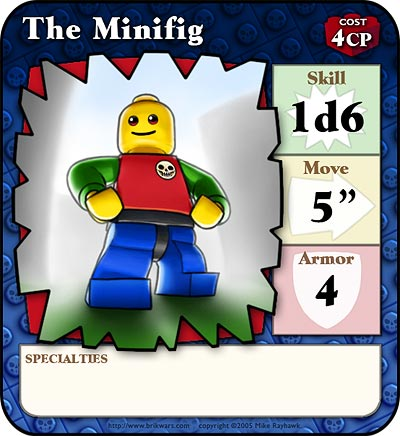
\includegraphics[width=2.78in]{minifig_color.jpg}
\end{figure}

\subsubsection{Trolls}

Trolls, or Goblins, Orcs or Trow are something of a brother race to Minis.  Outwardly their appearance is very similar to Minis, with roundish green heads instead of yellow.  Historically they occupy the western highlands of WesternHighlandStan, but like Minis they can be found in small numbers pretty much everywhere.  War between Trolls and Minis is so common it's pretty much the assumed state.

Breeder: Very High

Troll card

\begin{tabular}{|l|l|}
\multicolumn{2}{c}{\bf Troll (5 CP) } \\ \hline
Skill & 1d6 \\ \hline
Move & 5" \\ \hline
Armor & 1d6 \\ \hline
\multicolumn{2}{l} {Specialization:} \\
\multicolumn{2}{l} {Pilot (1 CP) } \\ \hline
\end{tabular}

\subsubsection{Dorfs}

This is a Dorf.  She is made of beard and alcohol.  All craftsdwarfship is of fine quality.  She has been quite content lately.  She admired a fine trap recently.  She has been satisfied at work lately.  She is a resident of the SkyWall mountain range.  She likes Onyx, Steel, and cows for their haunting moos.  She is often surly.  She isn't given to flights of  fancy.  She needs alcohol to get through the working day.  She likes working outdoors and grumbles only mildly at inclement weather.

Breeder: Medium

Dorf card

\begin{tabular}{|l|l|}
\multicolumn{2}{c}{\bf Dorf (6 CP) } \\ \hline
Skill & 1d6 + 1 \\ \hline
Move & 4" \\ \hline
Armor & 1d10 \\ \hline
\multicolumn{2}{l} {Specialization:} \\
\multicolumn{2}{l} {Heavy Arms Training (1 CP) } \\ \hline
\end{tabular}

\subsubsection{Dungans}

Dungans are occasionally described as the filth of the earth.  This isn't fair to the filth, which Dungans happen to admire and worship.  By nature Dungans are social and boisterous, shouting when they should whisper and stomping around where they should tread carefully.  The natural marching order for Dungans is just behind the largest army they can follow; this nets them both a safe place in combat (Dungans are natural cowards) and plenty of worthwhile leavings.  Dungans have a long and agglomerous history of building magnificently foetid tribal cities at secret locations in the worst bits of the southern swampland - and then inviting everyone they meet to join them there.

Breeder: Unfortunately high

\begin{tabular}{|l|l|}
\multicolumn{2}{c}{\bf Dungan (3 CP) } \\ \hline
Skill & 1d4 \\ \hline
Move & 4" \\ \hline
Armor & 1d6 \\ \hline
\end{tabular}

\subsubsection{Machine Men}

The Machine Men of the Great Desert are without a doubt the most enigmatic of the BrikWorld races.  Composed entirely of metal, each individual has only the merest spark of Life to sustain it.  The race as a whole is forced to continually scavenge for Loot to repair themselves as their bodies degrade around them.  

Breeder: N/A

\begin{tabular}{|l|l|}
\multicolumn{2}{c}{\bf Basic Drone (5 CP) } \\ \hline
Skill & 1d6 \\ \hline
Move & 5" \\ \hline
Armor & 1d6 \\ \hline
\multicolumn{2}{l} {Specialization:} \\
\multicolumn{2}{l} {Marksmanship (1 CP) } \\ \hline
\end{tabular}

\subsubsection{Bayounix}

Like the Dungans, Bayounix are native to the swamplands of the south.  Unlike the Dungans, they are worth a damn.  Bayounix are BrikWorld's most resourceful race, making do with less and doing without for more.  They farm what they can on what land they can in the swamp, use what they can find for as long as they can make it last, and generally just try to get through life by not being in anyone's way.  Most Bayounik technology looks cobbled together from scraps, and it often was.  Bayounik equipment generally consists of only a mask and a weapon, both heavily enchanted to the limit of the user's CP.

Rumors occasionally surface that there is a subrace of giant Bayounik warriors living freely in the Wild in the depth of the swamps. 

Bayounik card

Breeder: Average

\begin{tabular}{|l|l|}
\multicolumn{2}{c}{\bf Bayounik (4 CP) } \\ \hline
Skill & 1d6 \\ \hline
Move & 5" \\ \hline
Armor & 1d6 \\ \hline
\end{tabular}

\subsection{Monster Races}

Although players can incorporate monster races into their armies, most monsters will need to be tamed, enslaved, or will require some other method of control.  Clear it with your GM first.

Most Monster races pack their own heat in the form of natural weapons and equipment, which can be looted as any weapon can and 

\subsubsection{Death Beetles}

Death Beetles live underground in twisty hive warrens.  An average Death Beetle is about the size of a minifig, and possesses dangerous natural weapons.

\begin{tabular}{|l|l|}
\multicolumn{2}{c}{\bf Death Beetles (4 CP) } \\ \hline
Skill & 1d6 \\ \hline
Move & 4" \\ \hline
Armor & 1d10 \\ \hline

\multicolumn{2}{c}{\bf Natural Equipment } \\ \hline
\multicolumn{2}{c}{ Two 1" Weapons (2 CP each) } \\ \hline
\end{tabular}

\subsubsection{Undead}

Life can be a tenacious thing.  It doesn't like dying.  Sometimes, through mysticism, necromancy or sheer bloody mindedness, life sticks around in the form of undead.  The undead are alive but lack Life to stave off their deterioration, and so must continually devour life to stay afloat, a strange inversion of the Life-Loot relationship.  Undead never heal, only decay slower, so the life of any undead at best begins as a zombie and ends a skeleton.

The predatory instincts of undead can be temporarily tamed in the presence of a trained necromancer.  See Magic system for details.

\begin{tabular}{|l|l|}
\multicolumn{2}{c}{\bf Zombie Template (-1 CP) } \\ \hline
Skill & -2 \\ \hline
Move & -2" \\ \hline
Armor & +2 \\ \hline
\multicolumn{2}{l} {Specialization:} \\
\multicolumn{2}{l} {Infectious Bite (1 CP)} \\
\multicolumn{2}{l} {Shambling Movement (-1 CP) } \\ 
\multicolumn{2}{l} {Half Mind (Undead) (-1 CP) } \\ 
\multicolumn{2}{c}{  } \\
\multicolumn{2}{c}{\bf Natural Equipment } \\ \hline
\multicolumn{2}{c}{ One 1" Bite (2 CP) } \\ \hline
\end{tabular}

\begin{tabular}{|l|l|}
\multicolumn{2}{c}{\bf Skeleton Template (-2 CP) } \\ \hline
Skill & -2 \\ \hline
Move & +0" \\ \hline
Armor & +0 \\ \hline
\multicolumn{2}{l} {Specialization:} \\
\multicolumn{2}{l} {Half Mind (Undead) (-1 CP) } \\ \hline
\end{tabular}

\subsubsection{Dragons}

Dragons are an intriguing race with a very unique psychology.  Were they more sociable they might have been a player race, but dragons are individualistic and yet fiercely competitive.  Not really party material.  It's worth going into a little more detail about dragons' packrat instincts, which will prove useful later.

{\bf Dragons and Hoarding}

Dragons are famed for collecting Loot, even though they can't actually do anything with it.  They just gather it, pile it up in their caves, and then they friggin' sit on it until someone comes around to kill them.  Why do they bother with this?

In a word, sex.  All dragons prefer to be on top.

Dragons live a very long time, over which they grow several orders of magnitude more powerful.  If two dragons were to get into a fight over mating or any other power struggle, one of them would probably die very quickly and like as not neither dragon knows which it is beforehand.  If both dragons maintain giant piles of Loot (capped by their Life), it becomes easier and much safer to gauge each other's strength.  If the other dragon's hoard is much bigger than yours, he can probably kick your ass nine ways to Sunday.  If yours is bigger, invite him over for tea, let him get a look at {\it your} stash, and then tell him what you want him to do.

Because of the wide variety of dragons in BrikWorld, we're not going to bother with stats.  When you get a model, work out what it ought to be worth in CP according to BrikWars creation rules.

\subsubsection{Aberrations}

Life is not always picky enough to stick with a single race.  Multi-origin creatures, so-called "aberrations," are among BrikWorld's most terrifying and disturbing residents.  They may be dumb or intelligent, harmless or deadly, and anything in between.

\section{The Geography and Sociopolitical Layout of BrikWorld}

Figure: BrikWorld during the Wild

During the Wild, BrikWorld nations were not so much nations as individual communities loosely grouped by common culture, barely staving off the predations of the world at large.  WesternHighlandStan nomadic tribes were locked in internicine conflicts among each other and with the dwarves of the SkyWall, who huddle for safety in their forts.  GenericFantasyLand citizens lived in generic fantasy villages and DragonLand towns fought off endless swarms of powerful megabeasts, while 01 and Bayoutopia attempted to quietly keep to themselves.

The only truly safe nation is that of the coastal archipelago, which is able to tame its small islands to create semi-peaceful places for minis to exist.  The problem is getting there without being eaten by sea monsters or worse and once there, fighting for room.

Figure: BrikWorld during the Taming

The adventuring revolution sparked during the Taming affected every nation of BrikWorld to some degree.  What had been untamed wilderness was now economic opportunity.  With just a little methodical planning, the occasional trickle of powerful items became a reliable stream.  Areas that had been quaint medieval villages became military powerhouses virtually overnight.

The change was not good news for everyone.  Archipelago suffered an political inversion, going from one of the safest and most powerful nations to by far the poorest.  Its islands were already tapped out, and while abundant treasure existed on the ocean floor, its citizens had no way of reaching it.

Likewise, the people of DragonLand took a step backward in terms of national unity.  Dragons are intelligent, and well aware of their own instinctual desires.  The newly discovered connection between their treasure hoard and the land it came from led them to conclude, almost in unison, that it'd be better to own the land itself than just the fruits thereof.  That way they could gauge each other's strength with just a simple map without that tedious ``walking into an ambush" business.  The dragons established themselves as mayors and governers, each carving out a little fief for themselves and attempting to expand it by any means necessary.  DragonLand in the Taming resembles nothing so much as a heavily gerrymandered piece of territory, full of danger and (for its time) sophisticated political intrigue.

Far north of that, in WesterHighlandStan, a fresh bit of generic fantasy racism was stirring.  Since the average troll has a CP cost slightly higher than that of the average minifig they are, on the whole, somewhat more capable of using the better bits of loot generated by dungeon farming and gathered in the Wild.  The leaders of WesterHighlandStan embarked on a program to slowly but forcefully push the nation's troll population into other lands, mostly southward into the swamp and northward into GenericFantasyLand.

In return for having hundreds of incompetent nomadic refugees forced upon them, GenericFantasyLand adopted a more hostile stance toward WesterHighlandStan.  Scouts were replaced with raids, and spies became assassins.  Now and again there was talk of war, which naturally did nothing but make WesterHighlandStan tribes feel that their pogrom was justified.

To the dwarves of the SkyWall, none of this mattered much.  Driven by the knowledge that natural danger brought its own treasure, the dwarves barred their fortess doors, turned inward, and dug ever wider and deeper.  They would often brag to their rare visitors that it was possible to walk from the northernmost tip of the SkyWall to the southernmost end seven times, without ever seeing daylight or taking the same path twice.

Figure: BrikWorld during the Struggle

Once the Wild was won, the flow of the most powerful items slowed to a trickle, and eventually stopped completely.  Control of the now-artifacts became a hotly-contested issue, eventually escalating to a kind of cold war.  All nations continued to farm their own dungeons for mid-high level treasure, while simultaneously poaching other nations' highest-level dungeons and sending spies to shadow enemy patrols to find more.  

With no dangerous Wild to traverse, trade routes were able to stretch across the whole of BrikWorld.  Among the most profitable routes was the Orange Transparent Road, which ran from the highest peaks of the SkyWall, followed the WesternHighlandStan-GenericFantasyLand border, and  terminated at Archipelago.  The main trade good was rebreathers, spawned only in the mountains and sold for enormous sums of CP in Archipelago.  Those rebreathers enabled Archipelago to access its sunken wealth and once again become one of the most influential nations.  As a byproduct of the need to defend those resources, private ownership of boats and rebreathers was banned.  Being caught on the open water without a permit was a capital offence, though entrepreneurs of all nations dared to do it anyway.

The nation which changed the least during this time was WesternHighlandStan.  After five centuries of intermittent warfare with GenericFantasyLand they emerged the stronger of the two, which they interpreted as a vindication of their longstanding racism.  

GenericFantasyLand, in desperate response, turned to the darker arts to shore up its strength: necromancers, long persecuted for practicing their abilities, were offered a legal place in GenericFantasyLand armies.  The necromancers naturally were happy to oblige; nowhere are fresh corpses more plentiful than just after a battle.  It was sometimes said of GenericFantasyLand soldiers that "they're men of such device, you have to kill them twice!"

Things weren't much brighter in DragonLand.  A century ago one dragon, DragonEmperor, dreamed of something greater than being the sole sovereign of huge tracts of swampland. DragonEmperor instead spent her energies establishing a political, military and magical resources, while biding her time and watching.  At an opportune moment when power was perfectly balanced between a number of parties she struck, seizing control not just of a small spot of land like her brethren, but of the entire nation.  DragonLand then existed under a two-tier hierarchy: its citizens served some local dragon lord, who in turn served the Dragon Emperor.  But DragonEmperor wasn't wholly satisfied even then, and secretly positioned her pieces to wage unending war until the entire world was hers.

TODO: Bayounix and Machine Men fluff

\section{FFS, Get to the Actual Game Already}

Despite the complexity of the setting, the structure of a BrikWorld game is fairly simple: get a quest/goal, kill stuff, loot/get rewarded, upgrade forces.  Standard RPG fare.

\subsection{Get a Quest and Kill Stuff}

Questing is one of the most common elements in RPGs. Anyone who's played a computer RPG should be more than familiar with how they work.  Brief summary: ``Go get ye flask." ``Okay, here is ye flask." ``Take this reward for getting ye flask."  Pretty vanilla stuff.  

BrikWorld uses BrikWars for its combat system.  Detailed rules already exist at www.BrikWars.com, and are an entertaining read in their own right.  So we're mostly going to skip over them too.  

One addition we'd like to contribute to standard BrikWars combat is a simple XP system.  In each encounter, a unit which distinguishes itself in combat via Heroic deeds can (at the discretion of the GM) be given an extra Life CP after the battle.  Transparent 1x1 pips works great as markers for these.  Acts of bravery constituting Heroism include dispatching an enemy worth more CP than the unit in single combat, charging into battle to rescue a fallen comrade, holding off a stronger force until reinforcements can arrive, etc.  

Heroic CP doesn't contribute to a unit's abilities or how much Loot the unit can carry until it's been spent on upgrades (see: Upgrading Your Forces).  However, if the unit takes lethal damage and happens to have a spare Heroic CP, it can burn the CP to survive.  Therefore, keeping a spare CP or two around for emergencies is not a terrible idea.

\subsection{Get Money}

A BrikWorld party accrues wealth in two principle ways: by receiving it as a quest reward, and by taking it in the form of Loot.  The first manner is identical to how quest rewards work in just about any RPG, but the latter deserves a little elaboration.

\subsubsection{Loot is Temporary}

It's very probable that the players will always have Loot CP equal to or very near their Life CP, even before entering a dungeon.  There's always a need for more equipment or a bigger sword.  Any loot they're carrying over the max will begin to degrade as soon as they leave for town again.  The half-life for loot degradation is about one week.  This means that each week, the extra Loot CP will halve.  For example, say a party of 100 Life CP leaves a dungeon carrying 180 CP of Loot.  If town is two weeks away, they will arrive with 120 CP of Loot.  A surplus of 80 becomes a surplus of 40, then a surplus of 20.  

In order to meet this loss the players should decide which pieces of equipment to downgrade or destroy, but the GM gets to decide (if she wants) how any downgrades happen.  The players can also hire out a number of baggage handlers at a rate of 1 CP per two weeks.  Each handler can carry back 8 CP of Loot.

\subsubsection{Loot is Taxable}

BrikWorld is as familiar with taxes as it is with death.  Some nations call it taxing, for others it's "salvage fees" or "mandatory voluntary donations."  It all amounts to the same thing - you're rich, they're not rich enough, so they're going to do something about it.  The exact tax rate is up to the GM and will probably depend on how well the players fight, but there are some minor guidelines. 

The period with the highest taxes is the Taming.  During the Wild towns focused more on keeping their people alive, demanding Loot from the players only as compensation and donations.  On the other hand, players will probably have to bribe replacements with Loot CP.  During the Struggle taxes of raw CP are equally low (maybe 25\%), but governments will occasionally confiscate exceptionally cool weapons and conscript trained troops.  During the Taming, though, what towns and cities need more than anything is sheer mass of equipment.  To get it they charge obscene rates (75\%ish) for permission to delve their dungeons, and they can predict almost exactly how much CP the players ought to be able to Loot.  No, as a matter of fact they {\it don't} care that you weren't able to find all of the hidden chests.  They were there, and probably aren't anymore, so pay up.  If you want non-taxed income there's still some Wild left.

As in the real world, larger cities tend to have higher tax rates but offer more services in return compared to towns or villages.  Cities have a larger supply of rookie adventurers willing to join up for less equipment.  Cities tend to have more powerful mages, with higher caps on upgrades and abilities.  Cities often have dedicated special-use trainers like pilots and healers, who would otherwise have been forced to generalize.

\subsection{Upgrading Your Forces}

Assuming the players have any CP left over from the previous section, this is where they can spend it.

\subsubsection{Upgrading Units}

After a unit has accrued at least one Heroic CP, it can convert it in town or other places of safety into an upgrade for its abilities.  Through meditation, intense training and enough steroids to try out for the MBA, minifigs can empower themselves according to BrikWars custom creation rules.  They need no more aid than the accumulated CP for the upgrade. 

Sometimes, however, a mini needs a little more oomph than simple stat increases can provide.  Two later sections: Specialization and Magic, detail additional means of leveling.

\subsubsection{Upgrading Equipment}

\subsubsection{Recuiting Units}

\section {Magic}

\section {Crunch}
\subsection{Equipment}

In general, minifigs can equip at most five pieces of equipment: a weapon/shield in each hand, body armor, helmet, and a miscellaneous item.  

\subsection{Specialization}

Any skill a unit might have which alters BrikWorld rules or needs more than a name's worth of explanation is generally described through an entry in this section.  Some are features and some are flaws and a player should feel free to take either or both, providing she has the CP to blow and can at least halfass a reason why a normal minifig would become a zombie vampire angel sniper with a coke habit.

\subsubsection{Features}

\begin{tabular}{|l|c|} \hline
Heavy Arms Training & 1 CP \\ \hline
\end{tabular}

This unit thinks "over-compensation" is something lawyers use to determine their pay.  Years of practice with increasingly larger weapons have given him muscles like an ox, and weapon capabilities half a size larger.  He can dual-wield heavy weapons, or hold a two-handed weapon in one hand and a shield in the other.

\begin{tabular}{|l|c|} \hline
Finesse & 1 CP \\ \hline
\end{tabular}

For those who prefer not to clean-and-jerk their swords every morning, there's Finesse.  A unit with finesse enjoys a straight -1 Use modifier for all melee weapons and shields.

\begin{tabular}{|l|c|} \hline
Marksman & 1 CP \\ \hline
\end{tabular}

A marksman is more capable than her peers at hitting her target in difficult circumstances.  Marksmen take one less skill penalty from cover, and receive one more skill bonus when aiming.

\begin{tabular}{|l|c|} \hline
Sharpshooter & 1 CP \\ \hline
\multicolumn{2}{l} {Prerequisites: } \\
\multicolumn{2}{l} {Marksman } \\ \hline
\end{tabular}

Marksmen who continue developing their ranged abilities can upgrade to Sharpshooter.  Sharpshooters are skilled at picking the softest, most vulnerable bits of their target, resulting in a +1 damage modifier when firing ranged weapons.

\begin{tabular}{|l|c|} \hline
Pilot & 1 CP \\ \hline
\end{tabular}

On a vehicle or steed, where other minifigs must focus on either steering or firing weapons, the Pilot has the ability to do both simulataneously.  A Pilot ignores the usual Action cost for steering a vehicle or steed, leaving him free to use his Action for more destructive purposes.

\subsubsection{Flaws}

Specializations in this section have a negative CP cost and can be used to "pad out" a CP allotment into a larger number of weaker units.  Keep in mind that these flaws affect the total CP of equipment those characters can use as well.  Also, when applied to existing units, these flaws do not "free up" CP for other uses; the CP is simply lost.

\begin{tabular}{|l|c|} \hline
Half Mind (Undead) & -1 CP \\ \hline
\end{tabular}

This unit is undead.  Without a constant influx of necromantic magic (a -1 SP modifier to the maintainer's pool) or devouring the flesh of the living, this unit will deteriorate at a rate of 1 CP per week.  Also, without magical control (see: Magic) an undead unit's only priority is to kill and eat the nearest living creature it sees.

\begin{tabular}{|l|c|} \hline
Shambling Movement & -1 CP \\ \hline
\end{tabular}

This unit cannot maintain a regular pace, for whatever reason.  Instead of moving a number of inches equal to the unit's Move, roll 1dN (where N is the Move) and move up to that number instead.


\subsection{Chart Porn}

\section {Campaigning }

How a BrikWorld campaign is organized depends on time period it's set in:
\begin{itemize}
\item {\bf Wild:} A Wild setting most resembles conventional fantasy RPGs.  The PCs are the only ones with the freedom to move about.  Everyone else is desperately needed for village defense.  On the bright side, the PCs don't need to travel far at all to find something worth killing.  Of course, since this is the Wild, the thing they find might well kill them right back.  Treasure is plentiful but troop replacements are dear.  Consider letting your players bribe the townsfolk into joining you at equal CP costs: 4 CP of loot per rookie.  

Wild quests should involve small-scale defense issues: death beetles in the farmland, a small dragon threatening outlying farmers, lost heirlooms, that kind of thing.  A campaign revolving around securing and protecting a single town is perfect for a Wild setting.

Taxes are low in Wild settings, as villages are more concerned with people than stuff.  If the PCs manage to get their hands on some equipment that's better than they are, go ahead and let them use it for the week or two it remains uber.  

\item {\bf Taming:} During the Taming, towns are linking up and growing in strength.  Roads are reliable, but still not safe.  What once were villages are now towns, bursting at the seams with people in search of personal wealth.  Local authorities have begun to manage dungeons which the PCs can requisition, but must pay steep taxes to loot. Untaxed Wild still exists beyond the reaches of civilization, but is just as dangerous as ever.  

Taming quests take place at a slightly larger scale than Wild quests.  Roads will need clearing, merchants will need guarding, {\it everyone} thinks they know of some ancient treasure just out of reach.  Foreigners and other breeder races occasionally contact towns for trade or ransom.  Peace may need to be made between adjacent towns squabbling over dungeon rights.  Where Wild campaigns focus on sheer survival, Taming campaigns are all about knitting together the disparate towns into a unified whole.

\item {\bf Struggle:} BrikWorld in the Struggle relies more on intrigue and deceit than sheer strength of numbers.  Nations are fighting each other for the choicest loot (a bit like Mad Max) and are staving off all-out war by stockpiling powerful warriors wielding priceless artifacts while keeping other nations from knowing exactly how strong that really makes them (a bit like the Cold War).  Additionally, the rising land of Archipelago and the united Dragon Empire tend to worry just about everyone.

Struggle quests generally gain from having a bit of a spy theme, and from fitting into the bigger picture.  The players are almost certainly in the employ of some nation and directed to the general vicinity of another.  Their employers might send them to a town to discern how many of its residents are secretly Heroes, or to assassinate one, take whatever he's got and deliver it to a friendly Hero waiting just outside town.  Or, they might shadow an enemy patrol group to mark the location of unpublished dungeons, then raid the dungeon and return with the loot as quickly as possible.  Finally, if the players just want a simple dungeon crawl, Archipelago is still in the business of diving for treasures.  This provides an additional challenge from being gimped by the need to equip rebreathers while fending off Lovecraftian monstrosities.  

\end{itemize} 

\subsection{Quick Adventure Construction}

\section{Adventure Hooks}

\begin{itemize}

\item A local township has been getting reports of death beetles emerging from a dungeon several months earlier than they should, and send players to investigate (see sample quest below).

\item A SkyWall rocket ship suddenly fails and crash lands on the border of either WesternHighlandStan and GenericFantasyLand, or GenericFantasyLand and DragonLand.  The players are sent to capture or kill the Space Men and loot their ship, while preventing other nations from doing the same.

\item A local bandit group has recent been spotted wielding some Bayounik weaponry.  Players are sent to kill them and locate the trader who supplied them.

\item The players are lavishly hired by one dragon to steal some valuable loot from another.

\item The players must guard a GenericFantasyLand merchant as he travels to the SkyWall peaks for rebreathers, then takes them to Archipelago.

\item The players are invited to join in the underwater treasure hunt with the newly delivered rebreathers.

\item After releasing Dagon in the treasure hunt, the players must lure Him into another dungeon and hope whatever's there wipes him out and doesn't get curious.

\end{itemize}

\subsection{Sample Quest: "Just Another Bug Hunt"}

\section{Miscellaneous Screeds}
\subsection{Roleplaying + Wargaming = Rollplaying}
There is a great variety of roleplaying games available today.  Virtually all of them encourage or enforce a strict interpretation of roleplaying on the part of the players, namely first-person extemporaneous acting in response to in-game events.  Depending on the game this might only pertain to NPC interaction or might be the means by which every combat action is taken, but they all have it and they're all {\em serious} about it.  The easiest way to troll any diverse group of roleplayers is to strike up a conversation about how much roleplaying is "enough."  The word "rollplaying" itself arises from a common pejorative for people who are more interested in the combat and loot of the game than the narrative elements.

On the other side of the store, there's an equally wide variety of wargames.  While each system likely has a great deal of fluff about the setting and armies involved, there's almost never any justification for the actual fighting players do beyond "my guys hate his guys," nor narrative impacts because of it.  By far the most common persistent effects of a game are tournament standings and sour experiences, because wargames are also extremely competitive.  If you ever want a greater appreciation of your gaming buddies, ask any diverse group of wargamers for their horror stories.

BrikWorld exists in an attempt to find a happy medium, a combination of the two styles that takes the best from each without giving in to their respective excesses.  A story-driven RPG experience with combat-heavy wargaming mechanics.  A true rollplaying game.

\section {TODO}

Finish fluff

Get some goddamn names already

\begin{itemize}
\item Engardea
\item Sylvynon
\item Virovon
\end{itemize}


Finish the map

Do Magic system rough draft

Do crunch/equipment rough draft

Write out sample adventure

\end{document}


